\chapter{THỰC NGHIỆM VÀ ĐÁNH GIÁ}

\section{Thiết lập thực nghiệm}

Nhóm thực hiện ba loại kiểm tra: chạy các ví dụ nhỏ để quan sát từng bước INSERT/DELETE, đối chiếu kết quả với DBSCAN chạy lại, và đo chất lượng cụm cùng thời gian cập nhật trên luồng thẻ mô phỏng.

\begin{table}[H]
\centering
\caption{Các cấu hình chính trong thực nghiệm}
\label{tab:experiment_setup}
\normalsize
\begin{tabularx}{\textwidth}{@{}P{3.2cm}YP{3.5cm}@{}}
\toprule
\textbf{Thí nghiệm} & \textbf{Dữ liệu} & \textbf{Cấu hình} \\
\midrule
Ví dụ INSERT/DELETE & Các kịch bản 2D trong Chương 2 & Eps = 1,1; MinPts = 4 \\
Minh họa ATM & 1.200 tọa độ mô phỏng & Eps = 0,5 km; MinPts = 4 \\
So sánh trên luồng thẻ & D0 có 500 điểm; benchmark phát lại 20 cập nhật đầu & Eps = 0,4; MinPts = 6; 2D, 3D và 4D \\
\bottomrule
\end{tabularx}
\end{table}

DBSCAN và Incremental DBSCAN OOP là phần nhóm tự cài. DBSCAN, HDBSCAN và OPTICS của scikit-learn được dùng làm đối chứng \parencite{sklearnDBSCAN,sklearnHDBSCAN,sklearnOPTICS}. Trong benchmark luồng thẻ, bốn phương pháp nhận cùng dữ liệu đã chuẩn hóa, khoảng cách Euclidean và thứ tự cập nhật. Ba thuật toán thư viện được chạy lại trên toàn bộ dữ liệu hiện có sau mỗi cập nhật; bản Incremental DBSCAN xử lý INSERT/DELETE trên trạng thái đã lưu. Các tham số riêng của từng phương pháp được trình bày ở Chương 4, Bảng~\ref{tab:comparison_parameters}. Demo ATM 2D dùng tọa độ kilômét chưa chuẩn hóa và cấu hình riêng.

Benchmark thời gian chạy 5 lượt, có một lượt khởi động không tính vào kết quả. Mỗi lượt dùng cùng dữ liệu và cùng thứ tự 20 cập nhật, gồm 10 INSERT và 10 DELETE. Bảng thời gian báo trung vị và độ lệch chuẩn. Silhouette được tính trên trạng thái cuối của 20 cập nhật trong một lần chạy xác định, không phải trung bình của 5 lượt thời gian.

\section{Kết quả khi thêm điểm}

Các ví dụ INSERT dùng \(\mathrm{Eps}=1{,}1\), \(\mathrm{MinPts}=4\). Bốn trường hợp cho thấy một điểm mới có thể là nhiễu, tạo cụm mới, gia nhập cụm đang có hoặc làm các cụm nhập lại với nhau.

\begin{table}[H]
\centering
\caption{Kết quả các trường hợp INSERT}
\label{tab:insert_results}
\normalsize
\begin{tabularx}{\textwidth}{@{}P{2.4cm}YY@{}}
\toprule
\textbf{Trường hợp} & \textbf{Điều xảy ra} & \textbf{Kết quả sau cập nhật} \\
\midrule
Noise & Điểm mới không đủ lân cận và không nằm cạnh điểm lõi. & Điểm mới được đánh dấu nhiễu; cụm cũ giữ nguyên. \\
Creation & Điểm mới làm một số điểm đạt điều kiện lõi, nhưng chưa nối tới cụm cũ. & Các điểm liên quan tạo thành cụm mới. \\
Absorption & Điểm mới hoặc các điểm lân cận mới đạt điều kiện lõi trong vùng của một cụm cũ. & Cụm cũ được mở rộng; một số điểm nhiễu có thể thành điểm biên. \\
Merge & Các điểm lõi mới tạo đường nối giữa hai cụm cũ. & Các cụm có liên quan được gộp thành một cụm. \\
\bottomrule
\end{tabularx}
\end{table}

Trong ví dụ Merge, dữ liệu ban đầu có hai cụm. Điểm \(p\) được chèn vào giữa và làm các điểm ở hai phía trở thành lõi. Tập \(\mathrm{UpdSeed}_{Ins}\) chạm tới cả hai cụm, nên chương trình gộp chúng. Hình~\ref{fig:report_insert_merge} thể hiện các bước từ trước khi chèn đến sau khi cập nhật.

\begin{figure}[H]
    \centering
    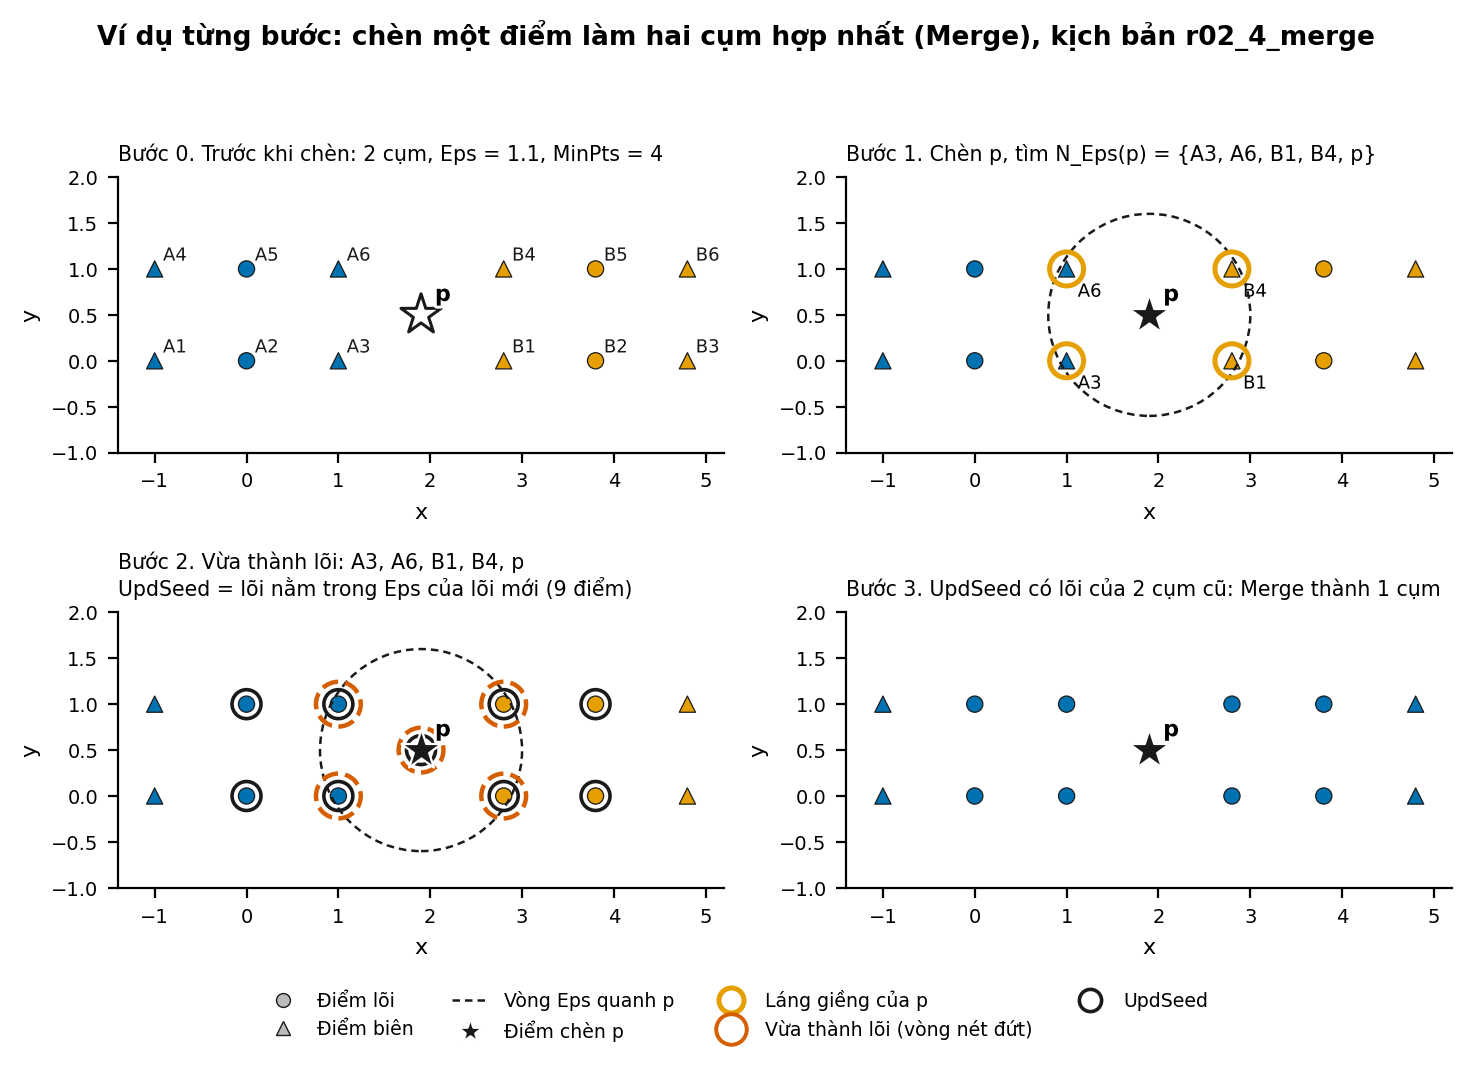
\includegraphics[width=0.98\textwidth]{Images/d05_steps_insert_merge.png}
    \caption{Các bước chèn điểm làm hai cụm nhập lại thành một cụm}
    \label{fig:report_insert_merge}
\end{figure}

\section{Kết quả khi xóa điểm}

Các ví dụ DELETE cũng dùng \(\mathrm{Eps}=1{,}1\), \(\mathrm{MinPts}=4\). Xóa một điểm không phải lúc nào cũng làm cụm bị tách. Kết quả phụ thuộc vào việc các điểm lõi còn giữ được đường nối hay không.

\begin{table}[H]
\centering
\caption{Kết quả các trường hợp DELETE}
\label{tab:delete_results}
\normalsize
\begin{tabularx}{\textwidth}{@{}P{2.8cm}YY@{}}
\toprule
\textbf{Trường hợp} & \textbf{Điều xảy ra} & \textbf{Kết quả sau cập nhật} \\
\midrule
Removal & Không còn seed lõi cần kiểm tra; có thể điểm bị xóa là lõi duy nhất của cụm. & Cụm có thể biến mất; các điểm còn lại thành nhiễu nếu không còn lõi nào. \\
Reduction & Các seed của cụm vẫn kề trực tiếp nhau. & Cụm không bị tách, dù một số điểm có thể mất trạng thái lõi và trở thành biên. \\
Potential Split - Split & BFS từ các seed không tìm được đường qua điểm lõi để nối các phía. & Cụm cũ tách thành nhiều cụm; điểm không còn cạnh lõi có thể thành nhiễu. \\
Potential Split - Non-split & Có đường nối thay thế qua các điểm lõi khác. & Cụm vẫn giữ nguyên, dù điểm cầu nối ban đầu đã bị xóa. \\
\bottomrule
\end{tabularx}
\end{table}

Ví dụ Split bắt đầu với một cụm có điểm \(p\) nối hai phía. Sau khi xóa \(p\), BFS không tìm được đường qua các điểm lõi giữa hai phía, nên cụm tách làm hai và điểm \(I\) trở thành nhiễu. Hình~\ref{fig:report_delete_split} minh họa kết quả này.

\begin{figure}[H]
    \centering
    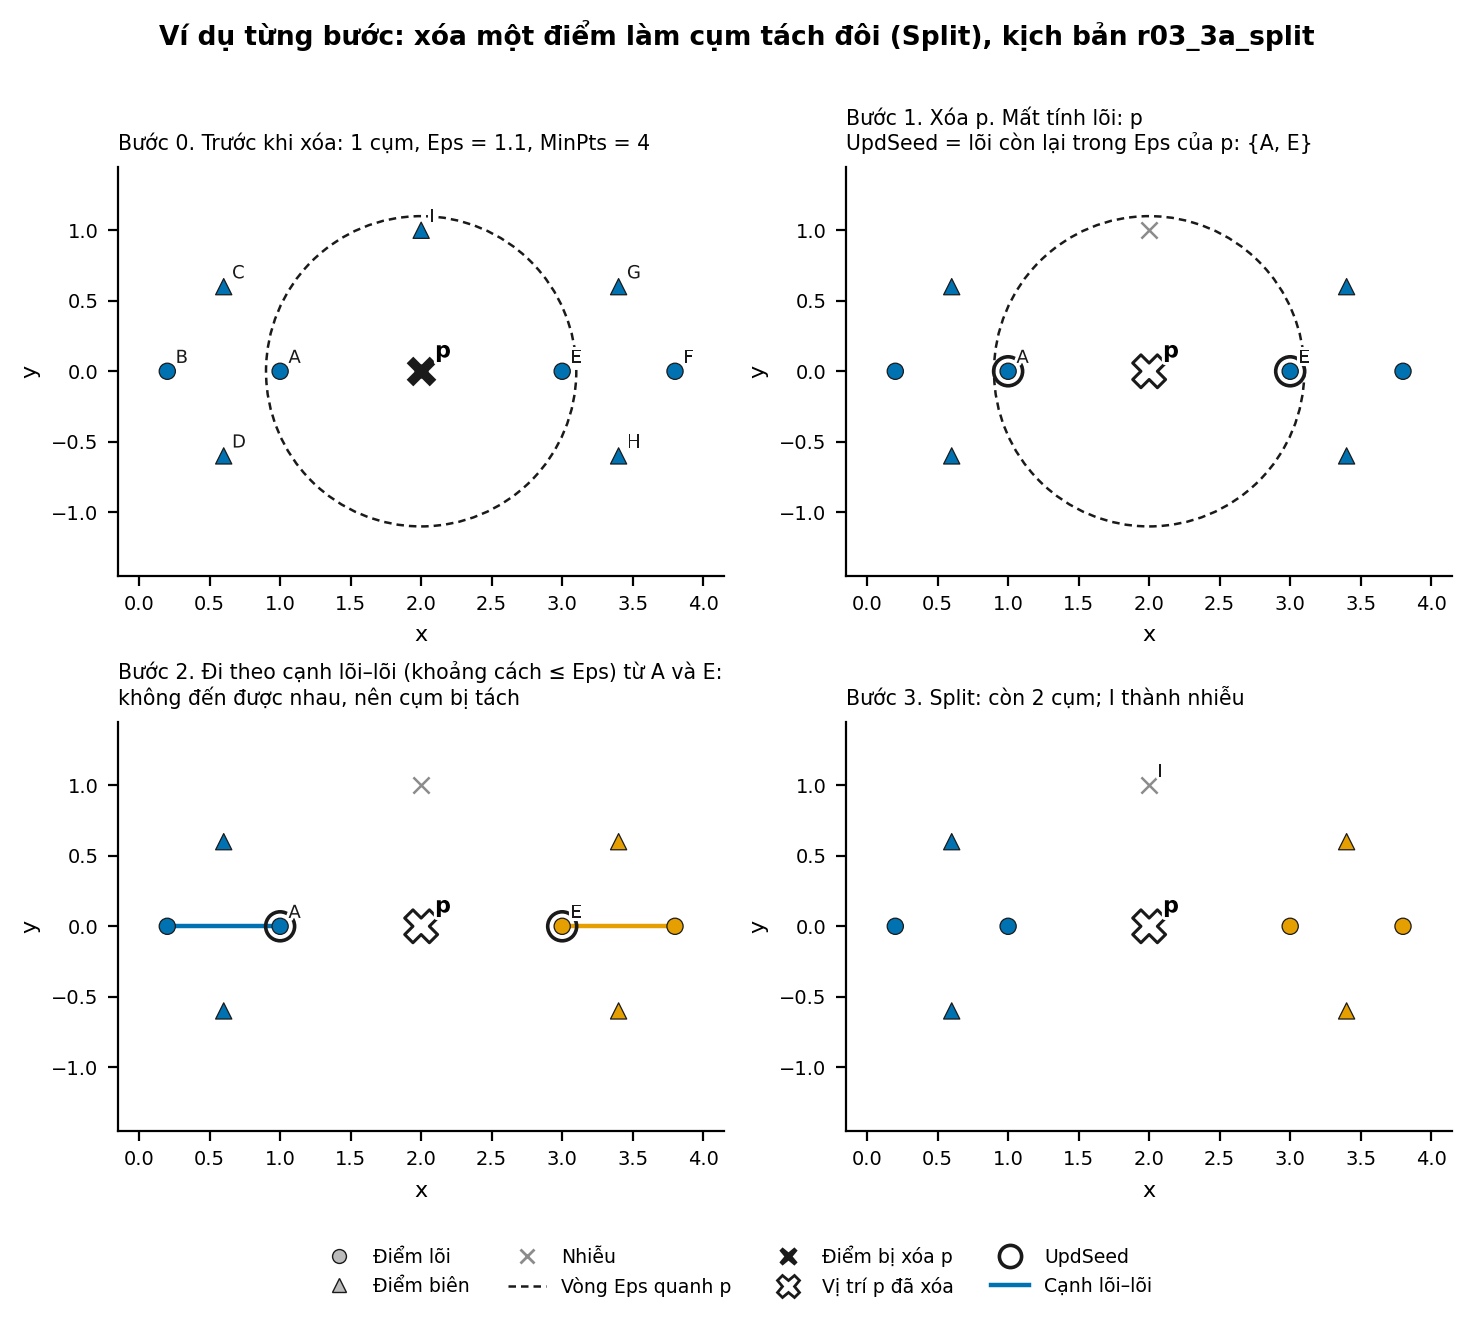
\includegraphics[width=0.98\textwidth]{Images/d06_steps_delete_split.png}
    \caption{Các bước xóa điểm cầu nối làm một cụm tách thành hai cụm}
    \label{fig:report_delete_split}
\end{figure}

Ở trường hợp Non-split, sau khi xóa điểm cầu nối ban đầu vẫn còn một đường đi qua các điểm lõi. Vì vậy BFS xác nhận các seed vẫn thuộc cùng một thành phần và không tách cụm. Hai trường hợp này cho thấy chỉ biết một điểm lõi bị xóa là chưa đủ; cần kiểm tra các đường nối còn lại.

\section{Minh họa trên không gian 2D}

Các ví dụ Merge và Split ở trên dùng tọa độ 2D để có thể theo dõi trực tiếp điểm mới, điểm bị xóa, vòng Eps và các điểm trong \(\mathrm{UpdSeed}\). Notebook minh họa trình bày từng bước của hai ví dụ này, sau đó chạy DBSCAN trên 1.200 tọa độ ATM.

Với ATM 2D, cấu hình Eps = 0,5 km và MinPts = 4 tạo ra 6 cụm, 142 điểm nhiễu; Silhouette tự cài trên các điểm không nhiễu là 0,3362. Các phương pháp nhận cùng hai tọa độ và khoảng cách Euclidean. DBSCAN dùng \texttt{eps=0.5, min\_samples=4}; HDBSCAN dùng \texttt{min\_cluster\_size=4, min\_samples=4} vì thuật toán này không có Eps; OPTICS dùng \texttt{min\_samples=4, eps=0.5, max\_eps=0.500001} và trích cụm theo kiểu DBSCAN. Vì Silhouette bỏ điểm nhiễu, nhóm đọc chỉ số này cùng số cụm và tỷ lệ nhiễu, không dùng riêng nó để kết luận mô hình nào tốt hơn.

\section{Đối chiếu với DBSCAN chạy lại}

Để kiểm tra phép cập nhật, nhóm so sánh trạng thái của Incremental DBSCAN với DBSCAN của scikit-learn được fit lại trên cùng tập điểm sau mỗi thao tác. Phép đối chiếu xét phân hoạch cụm, trạng thái lõi và điểm nhiễu; mã nhãn cụm có thể khác nhau nhưng cách chia điểm phải tương ứng.

Trong kết quả lưu tại \texttt{results/equivalence\_results.csv}, có 317 lần đối chiếu: 9 lần fit ban đầu, 154 INSERT và 154 DELETE. Cả 317 lần đều đạt điều kiện tương đương; không có trường hợp sai khác được ghi nhận. Kết quả này gồm các ví dụ cập nhật và luồng thẻ, cho thấy các trạng thái đã kiểm tra của bản OOP khớp với DBSCAN chạy lại.

Đây là kiểm tra trên các bộ dữ liệu và thao tác hiện có, không chứng minh thuật toán đúng với mọi dữ liệu có thể gặp.

\section{So sánh chất lượng cụm bằng Silhouette}

Nhóm tự cài Silhouette và dùng chỉ số này làm cách đánh giá chất lượng cụm chính. Điểm nhiễu bị bỏ khỏi phép tính, nên bảng luôn kèm số cụm và tỷ lệ nhiễu. ARI được dùng riêng để kiểm tra mức độ đồng thuận giữa hai cách cài DBSCAN, không dùng để xếp hạng HDBSCAN hay OPTICS.

Trên ATM 2D, các phương pháp cho kết quả sau:

\begin{table}[H]
\centering
\caption{So sánh Silhouette trên dữ liệu ATM 2D}
\label{tab:atm_silhouette}
\normalsize
\begin{tabularx}{\textwidth}{@{}Yccc@{}}
\toprule
\textbf{Phương pháp} & \textbf{Silhouette} & \textbf{Số cụm} & \textbf{Tỷ lệ nhiễu} \\
\midrule
Incremental DBSCAN OOP & 0,3362 & 6 & 11,83\% \\
scikit-learn DBSCAN & 0,3362 & 6 & 11,83\% \\
scikit-learn HDBSCAN & 0,3978 & 23 & 9,92\% \\
scikit-learn OPTICS & 0,3362 & 6 & 11,83\% \\
\bottomrule
\end{tabularx}
\end{table}

HDBSCAN có Silhouette cao hơn trong cấu hình này nhưng đồng thời tạo ra 23 cụm, nhiều hơn đáng kể so với sáu cụm của các phương pháp còn lại. Vì vậy, không thể chỉ nhìn điểm Silhouette rồi kết luận HDBSCAN tốt hơn; cần xem số cụm, tỷ lệ nhiễu và mục tiêu của bài toán.

Trên luồng thẻ, bảng dưới tính tại trạng thái cuối sau 20 cập nhật. Cả bốn phương pháp cho cùng 3 cụm và 1\% điểm nhiễu trong ba lát đặc trưng đang thử.

\begin{table}[H]
\centering
\caption{Silhouette trên các lát 2D, 3D và 4D của luồng thẻ}
\label{tab:card_silhouette}
\normalsize
\begin{tabularx}{\textwidth}{@{}ccccY@{}}
\toprule
\textbf{Số chiều} & \textbf{Silhouette} & \textbf{Số cụm} & \textbf{Nhiễu} & \textbf{Ghi chú} \\
\midrule
2D & 0,7785 & 3 & 1\% & Bốn phương pháp cho cùng phân hoạch trong cấu hình này. \\
3D & 0,7839 & 3 & 1\% & Bốn phương pháp cho cùng phân hoạch trong cấu hình này. \\
4D & 0,7463 & 3 & 1\% & Bốn phương pháp cho cùng phân hoạch trong cấu hình này. \\
\bottomrule
\end{tabularx}
\end{table}

Các lát 2D, 3D và 4D được lấy từ cùng một luồng dữ liệu, nên không phải ba bộ dữ liệu độc lập. Kết quả giống nhau giữa bốn phương pháp chỉ áp dụng cho dữ liệu, tham số và 20 cập nhật này; không có nghĩa các thuật toán luôn cho cùng kết quả.

\section{Thời gian chạy và giới hạn đo đạc}

Bảng~\ref{tab:update_runtime} báo tổng thời gian của 20 cập nhật, lấy trung vị \(\pm\) độ lệch chuẩn qua 5 lượt. Đơn vị là mili giây.

\begin{table}[H]
\centering
\caption{Thời gian cập nhật trên 20 thao tác}
\label{tab:update_runtime}
\normalsize
\begin{tabularx}{\textwidth}{@{}cYYYY@{}}
\toprule
\textbf{Dữ liệu} & \textbf{Incremental OOP} & \textbf{sklearn DBSCAN} & \textbf{sklearn HDBSCAN} & \textbf{sklearn OPTICS} \\
\midrule
Thẻ 2D & 321,08 \(\pm\) 25,53 & 136,72 \(\pm\) 14,81 & 198,41 \(\pm\) 18,84 & 14.571,56 \(\pm\) 238,01 \\
Thẻ 3D & 288,78 \(\pm\) 20,95 & 148,09 \(\pm\) 6,57 & 194,18 \(\pm\) 19,08 & 13.824,08 \(\pm\) 373,53 \\
Thẻ 4D & 194,56 \(\pm\) 9,98 & 152,03 \(\pm\) 8,23 & 208,37 \(\pm\) 22,12 & 13.485,85 \(\pm\) 232,03 \\
\bottomrule
\end{tabularx}
\end{table}

Trong phép đo này, DBSCAN scikit-learn fit lại có tổng thời gian thấp hơn bản OOP ở cả ba số chiều. HDBSCAN cũng nhanh hơn ở 2D và 3D, còn bản OOP thấp hơn một chút ở 4D. OPTICS có thời gian cao nhất trong cả ba cấu hình. Kết quả này không cho thấy Incremental DBSCAN luôn nhanh hơn cách fit lại; hình~\ref{fig:runtime_benchmark} thể hiện chênh lệch trên thang log.

\begin{figure}[H]
    \centering
    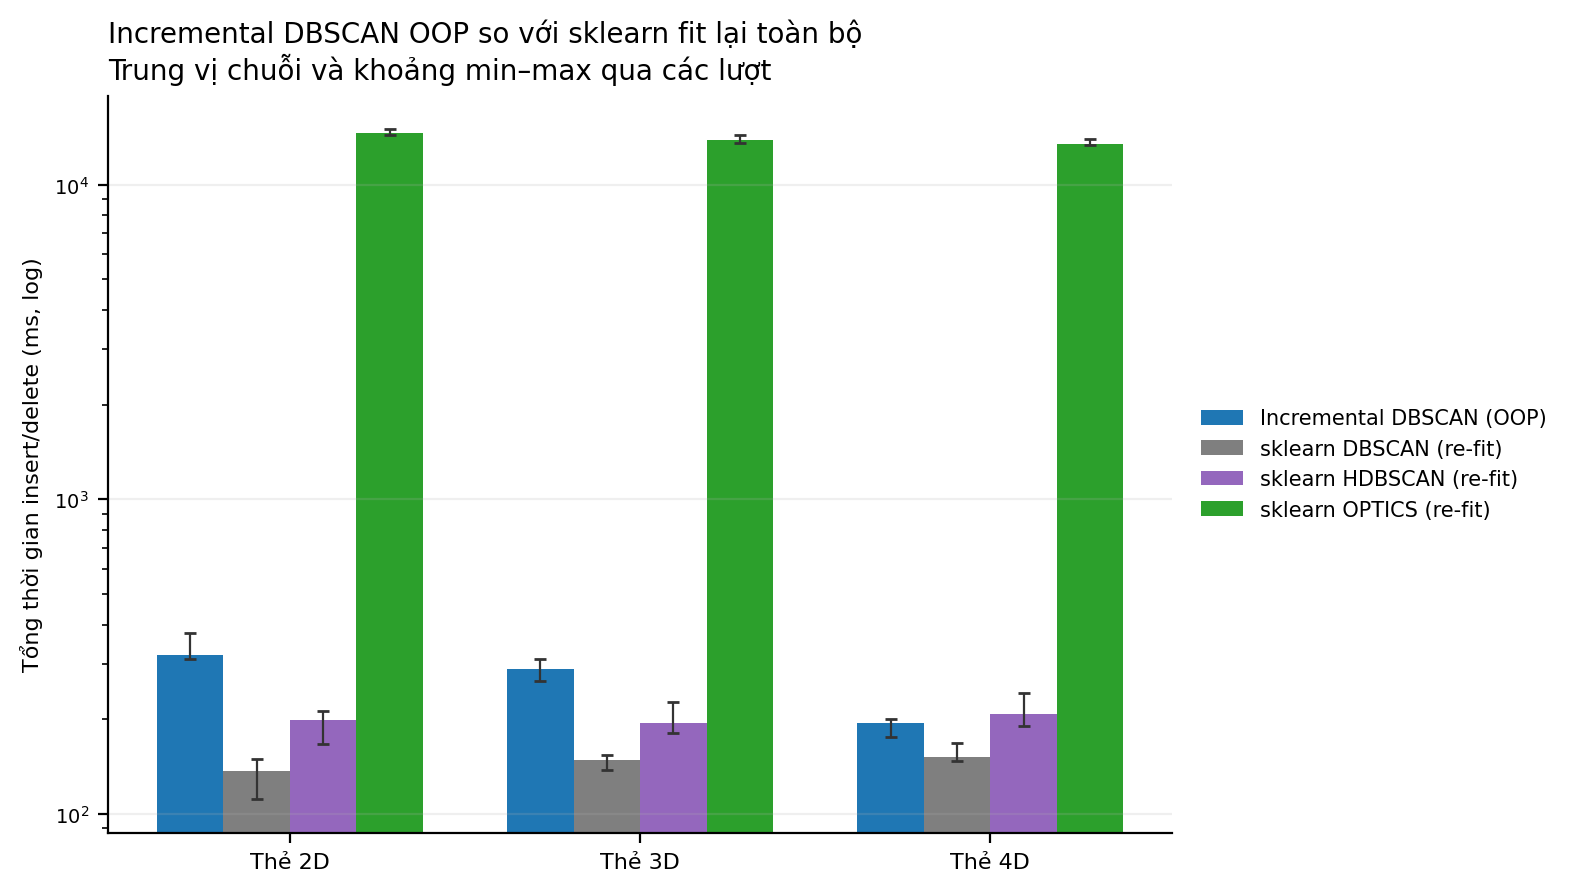
\includegraphics[width=0.9\textwidth]{Images/density_algorithm_benchmark.png}
    \caption{Tổng thời gian cập nhật qua 5 lượt benchmark}
    \label{fig:runtime_benchmark}
\end{figure}

Tuy vậy, thời gian fit ban đầu D0 của bản OOP cao hơn DBSCAN scikit-learn. Bảng~\ref{tab:initial_fit_runtime} tách riêng bước này để tránh chỉ nhìn thời gian cập nhật rồi kết luận bản OOP nhanh hơn trong toàn bộ quá trình.

\begin{table}[H]
\centering
\caption{Thời gian fit ban đầu D0, trung vị qua 5 lượt (ms)}
\label{tab:initial_fit_runtime}
\normalsize
\begin{tabularx}{\textwidth}{@{}cYYYY@{}}
\toprule
\textbf{Dữ liệu} & \textbf{Incremental OOP} & \textbf{sklearn DBSCAN} & \textbf{sklearn HDBSCAN} & \textbf{sklearn OPTICS} \\
\midrule
Thẻ 2D & 1.315,57 & 8,22 & 10,53 & 697,82 \\
Thẻ 3D & 1.288,58 & 7,75 & 10,46 & 701,88 \\
Thẻ 4D & 1.434,08 & 9,42 & 13,32 & 693,52 \\
\bottomrule
\end{tabularx}
\end{table}

Nhóm không đo bộ nhớ thành một thí nghiệm riêng. Phần này chỉ nhận xét định tính rằng Incremental DBSCAN phải lưu thêm lân cận và trạng thái điểm để dùng lại khi cập nhật. Thời gian nêu trên cũng chỉ phản ánh môi trường chạy, dữ liệu mô phỏng và 20 cập nhật đầu; không đại diện cho toàn bộ 300 cập nhật hay dữ liệu giao dịch thật.

\section{Nhận xét chung}

Các ví dụ nhỏ giúp quan sát rõ việc thêm điểm có thể tạo hoặc gộp cụm, còn xóa điểm có thể làm cụm giảm, biến mất hoặc tách ra. Kết quả đối chiếu hiện có không ghi nhận sai khác giữa Incremental DBSCAN và DBSCAN chạy lại. Trong benchmark thẻ, DBSCAN scikit-learn fit lại nhanh hơn bản OOP ở cả ba số chiều; HDBSCAN nhanh hơn ở 2D/3D và chậm hơn một chút ở 4D. Bước fit ban đầu của bản OOP cũng chậm hơn các phương pháp thư viện. Vì vậy, thí nghiệm hiện tại xác nhận tính đúng của cập nhật, nhưng chưa cho thấy lợi thế thời gian của bản OOP trên prefix 20 thao tác này.